\section{Results and discussion}
\label{sec:results}
%************************************************

\subsection{Experiments}
\label{subsec:experiments}

%\InsTab{tables/05sinterTableExperimental}
Initially, experimental values identifying the bulk behavior, $\phi_{e-psh}$, 
$\phi_{e-sh}$ and $\rho_{b}$, for sinter fine have been acquired though the
SRSCT, see Table \ref{tab:05sinterTableExperimental}.
\begin{table}[h]
\centering
\begin{tabular}{cccccc}
\hline
$\sigma_n$ (Pa) & $\tau$ (Pa) & $\mu_{psh}$ (-) & $\tau_{\%}$ (\%) &
$\mu_{sh}$ (-) & $\rho_b$ (kg/m3) \\
\hline
    1068  & 1059  & 0.9916 & 80 & 1.2333 & 1718 \\
    2069  & 1818  & 0.8787 & 80 & 0.9994 & 1759 \\
    10070 & 8232  & 0.8175 & 80 & 1.1712 & 1802 \\

\hline
\end{tabular}
\caption[Experimental results]{Experimental results. Values for three
load conditions}
\label{tab:05sinterTableExperimental}
\end{table}
Later, two AOR test have been performed, given an average angle of $38.85
^\circ$.
 
ONE TABLE FOR EACH MATERIAL

% a
% 
% \begin{equation}
F_{t,ij} \leq \mu_s F_{n,ij},
 \label{eq:force_t}
\end{equation}


\subsection{DEM Simulations}
\label{subsec:simulations}
% \lipsum[1]
% \begin{equation}
\begin{aligned}
	k_n &= \frac{4}{3} E_{eq} \sqrt{R_{eq} \xi_n} ,\\
	\gamma_n &= 2 \sqrt{\frac{5}{6}} \beta \sqrt{S_n m_{eq}} ,\\
	k_t &= 8 G_{eq} \sqrt{R_{eq}} \xi_n ,\\
	\gamma_t &= 2 \sqrt{\frac{5}{6}} \beta \sqrt{S_t m_{eq}} .
\end{aligned}
\label{eq:hertz}
\end{equation}

For sinter fine 704 shear cell and 54 static angle of repose simulations have
been realized with the variation described in Table \ref{tab:07DEMinputvalues},
gaining four values identifying the numerical bulk behavior, $\phi_{e-psh}$, 
$\phi_{e-sh}$, $AOR$ and $\rho_{b}$ for each simulated combination.
The shear cell simulations made are more than the angle of repose to account for
the different normal load applied.
\begin{table}[h]
\centering
\begin{tabular}{c|c|c|c|c}
\hline
average & std dev & average & DEM   & DEM \\
particle & particle & particle & Young's & Poisson's \\
    radius & radius & density & modulus & ratio \\
    [mm]  & [mm]  & [kg/m3] & [Gpa] & [-] \\
    \hline
    0.732 & 0.41  & 2500 - 3000 - 3500 & 10    & 0.40 \\
    \hline
    DEM   & DEM   & DEM   & constant & simulation \\
    sliding & rolling & coefficient & ring  & domain diameter \\
    friction & friction & restitution & velocity & to particle mean \\
    [-]   & [-]   & [-]   & [mm/s] & diameter ratio \\
    \hline
    0.4 - 0.6 - 0.8 & 0.4 - 0.6 - 0.8 & 0.5 - 0.7 - 0.9 & 2.196 & 20 - 36 - 38 - 40 \\

\hline
\end{tabular}
\caption{DEM input values}
\label{tab:07DEMinputvalues}
\end{table}


\subsection{ANN model development}
\label{subsec:annmodeldev}

We then fed the $NN$ with the same $DEM-micro$ parameters of these simulations
as input.
A series of NN have been realized for each bulk behavior as target, ranging from
5 to 40 neurons in the hidden layer.
The linear relationship between the
training values have been evaluated in Table \ref{tab:06inputRelationshipTable}.
\begin{table}[h]
\centering
\scalebox{1.0}{
\begin{tabular}{c|cccccccc}
\hline
          & $\mu_s$ & $\mu_r$ & $COR$ & $\rho_p$ & $\mu_{sh}$ & $\mu_{psh}$ & $\rho_{b}$ & $AOR$ \\
          \hline
    $\mu_s$ & 100.00 & 0.55  & 0.04  & 0.00  & 3.84  & 87.26 & 8.39  & 49.48 \\
    $\mu_r$ & 0.55  & 100.00 & 0.15  & 0.00  & 58.92 & 33.70 & 3.10  & 60.20 \\
    $COR$ & 0.04  & 0.15  & 100.00 & 0.00  & 15.52 & 0.57  & 1.71  & 0.00 \\
    $\rho_p$ & 0.00  & 0.00  & 0.00  & 100.00 & 4.98  & 5.71  & 99.00 & 0.00 \\
    $\mu_{sh}$ & 3.84  & 58.92 & 15.52 & 4.98  & 100.00 & 26.03 & 9.52  & 0.00 \\
    $\mu_{psh}$ & \textbf{87.26} & 33.70 & 0.57  & 5.71  & 26.03 & 100.00 & 4.33 
    & 0.00
    \\
    $\rho_{b}$ & 8.39  & 3.10  & 1.71  & \textbf{99.00} & 9.52  & 4.33  & 100.00
    & 0.00 \\
    $AOR$ & 49.48 & \textbf{60.20} & 0.00  & 0.00  & 0.00  & 0.00  & 0.00  &
    100.00 \\
    
\hline
\end{tabular}}
\caption{Values of linear relationship between considered variables multiplied
for 100}
\label{tab:06inputRelationshipTable}
\end{table}
EVALUTE IF ADD AOR AS ENTRY IN THE TABLE OR MAKE A NEW SEPARATE TABLE



% \lipsum[1]
% \begin{equation}
 \mu_r =  \tan(\iota) .
\label{equ:mur}
\end{equation}


\subsection{ANN identification}
\label{subsec:annmodeliden}
Subsequently, we controlled the square regression error between the $bulk-macro$
behavior in these simulations and in the output of the $NN$, see Eq.
\ref{eq:rsquare}.
\begin{equation}
R^2 = \frac {SSR}{SST} = 1 - \frac {SSE}{SST} .
 \label{eq:rsquare}
\end{equation}

SSE is the sum of squared error, SSR is the sum of squared regression, SST is
the sum of squared total.
As in literature, this goal has been achieved by first excluding 15\% of the
simulations from the training processes.\\

RMSE amplifies and severely punishes large errors, see Eq.
\ref{eq:rootMeanSquareError}.
\begin{equation}
RMSE = \sqrt{\frac{\sum _{i=1}^{n} (x_{i}-\widehat{x}_{i})^{2}}{n}}
\label{eq:rootMeanSquareError}
\end{equation}


Finally, we selected for each $bulk-macro$ behavior property ($\mu_{ie-ps}$, $\mu_{ie-s}$ and $\rho_b$) the $NN$ with the 
number of neurons that provided the maximum $R^2$.


% \lipsum[1]
% \begin{equation}
m \ddot{x}_{ij} + c \dot{x}_{ij} + k x_{ij} =  F_{ij} .
\label{equ:newtonlaw}
\end{equation}


\subsection{ANN application}
\label{subsec:annapplication}

Later, each of these three trained $NN$ received as insertion $100M$ different
combinations $DEM-micro$ parameters.
So, we gained the numerical bulk behavior for each of this combination. 
We then compared the values of these behaviors against the experimental bulk
values, $SRSCT$ and $AOR$, obtaining a narrow range of valid DEM-micro
combinations (about 80K).
These results have been showed through radar plots (Figs. \ref{fig:15Schulze}
and \ref{fig:16aorSchulzeIntersectionWorking}).
To highlight an eventual $clumping$ behavior, we also plot the results in a
cloud shape, see Fig. \ref{fig:17aorSchulzeIntersectionCloudSFRFCOR}.

%\begin{figure}[!htb] 
\centering 
\includegraphics[width=1.0\textwidth]{images/original/14aorSchulzeIntersection} 
\caption{aor Schulze Intersection}
\label{fig:14aorSchulzeIntersection} 
\end{figure}


% \begin{figure}[htp]
%     \centering
%     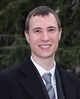
\includegraphics[width=.2\textwidth]{images/vitae/lbenvenuti}
%     \caption{OpenMP, MPI, MPI/OpenMP Hybrid runs of Box in a box testcase on 32
%     cores. The OpenMP-only run suffers from limited memory bandwidth in
%     memory-bound algorithms inside of the Modify section of the code. MPI-only has
%     low averaged runtimes for each section, but a very large Other timing, which
%     hints for a large amount of load-imbalance. Hybrid timings are a bit worse
%     on average, but because of better balancing, processes have lower wait times
%     inside of Other timing.}
% 	\label{fig:boxInBoxComparison}

\begin{figure}[!htb] 
\centering 
\includegraphics[width=.8\textwidth]{images/original/15Schulze} 
\caption{aor Schulze Intersection}
\label{fig:14aorSchulzeIntersection} 
\end{figure}


% \begin{figure}[htp]
%     \centering
%     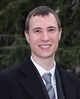
\includegraphics[width=.2\textwidth]{images/vitae/lbenvenuti}
%     \caption{OpenMP, MPI, MPI/OpenMP Hybrid runs of Box in a box testcase on 32
%     cores. The OpenMP-only run suffers from limited memory bandwidth in
%     memory-bound algorithms inside of the Modify section of the code. MPI-only has
%     low averaged runtimes for each section, but a very large Other timing, which
%     hints for a large amount of load-imbalance. Hybrid timings are a bit worse
%     on average, but because of better balancing, processes have lower wait times
%     inside of Other timing.}
% 	\label{fig:boxInBoxComparison}

% \lipsum[1]
\begin{figure}[!htb] 
\centering 
\includegraphics[width=.96\textwidth]{images/original/16aorSchulzeIntersectionWorking} 
\caption{aor Schulze Intersection working}
\label{fig:16aorSchulzeIntersectionWorking} 
\end{figure}


% \begin{figure}[htp]
%     \centering
%     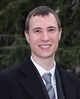
\includegraphics[width=.2\textwidth]{images/vitae/lbenvenuti}
%     \caption{OpenMP, MPI, MPI/OpenMP Hybrid runs of Box in a box testcase on 32
%     cores. The OpenMP-only run suffers from limited memory bandwidth in
%     memory-bound algorithms inside of the Modify section of the code. MPI-only has
%     low averaged runtimes for each section, but a very large Other timing, which
%     hints for a large amount of load-imbalance. Hybrid timings are a bit worse
%     on average, but because of better balancing, processes have lower wait times
%     inside of Other timing.}
% 	\label{fig:boxInBoxComparison}

% \begin{equation}
\begin{aligned}
\phi_{e-psh} &= \arctan \left(\frac{\tau_{psh}}{\sigma_{n,psh}} \right) ,\\
\mu_{psh} &=\tan(\phi_{e-psh}) .
\end{aligned}
 \label{eq:phi_ps}
\end{equation}

\begin{figure}[!htb] 
\centering 
\includegraphics[width=.96\textwidth]{images/original/17aorSchulzeIntersectionCloudSFRFCOR} 
\caption{Cloud aor Schulze Intersection working}
\label{fig:17aorSchulzeIntersectionCloudSFRFCOR} 
\end{figure}


% \begin{figure}[htp]
%     \centering
%     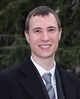
\includegraphics[width=.2\textwidth]{images/vitae/lbenvenuti}
%     \caption{OpenMP, MPI, MPI/OpenMP Hybrid runs of Box in a box testcase on 32
%     cores. The OpenMP-only run suffers from limited memory bandwidth in
%     memory-bound algorithms inside of the Modify section of the code. MPI-only has
%     low averaged runtimes for each section, but a very large Other timing, which
%     hints for a large amount of load-imbalance. Hybrid timings are a bit worse
%     on average, but because of better balancing, processes have lower wait times
%     inside of Other timing.}
% 	\label{fig:boxInBoxComparison}

